\begin{frame}{Solution: Batch Norm Layer}
	\begin{itemize}
		\item It is used to \tc{keywords}{normalize} the data.
	\end{itemize}
	\begin{figure}[H]
		\centering
		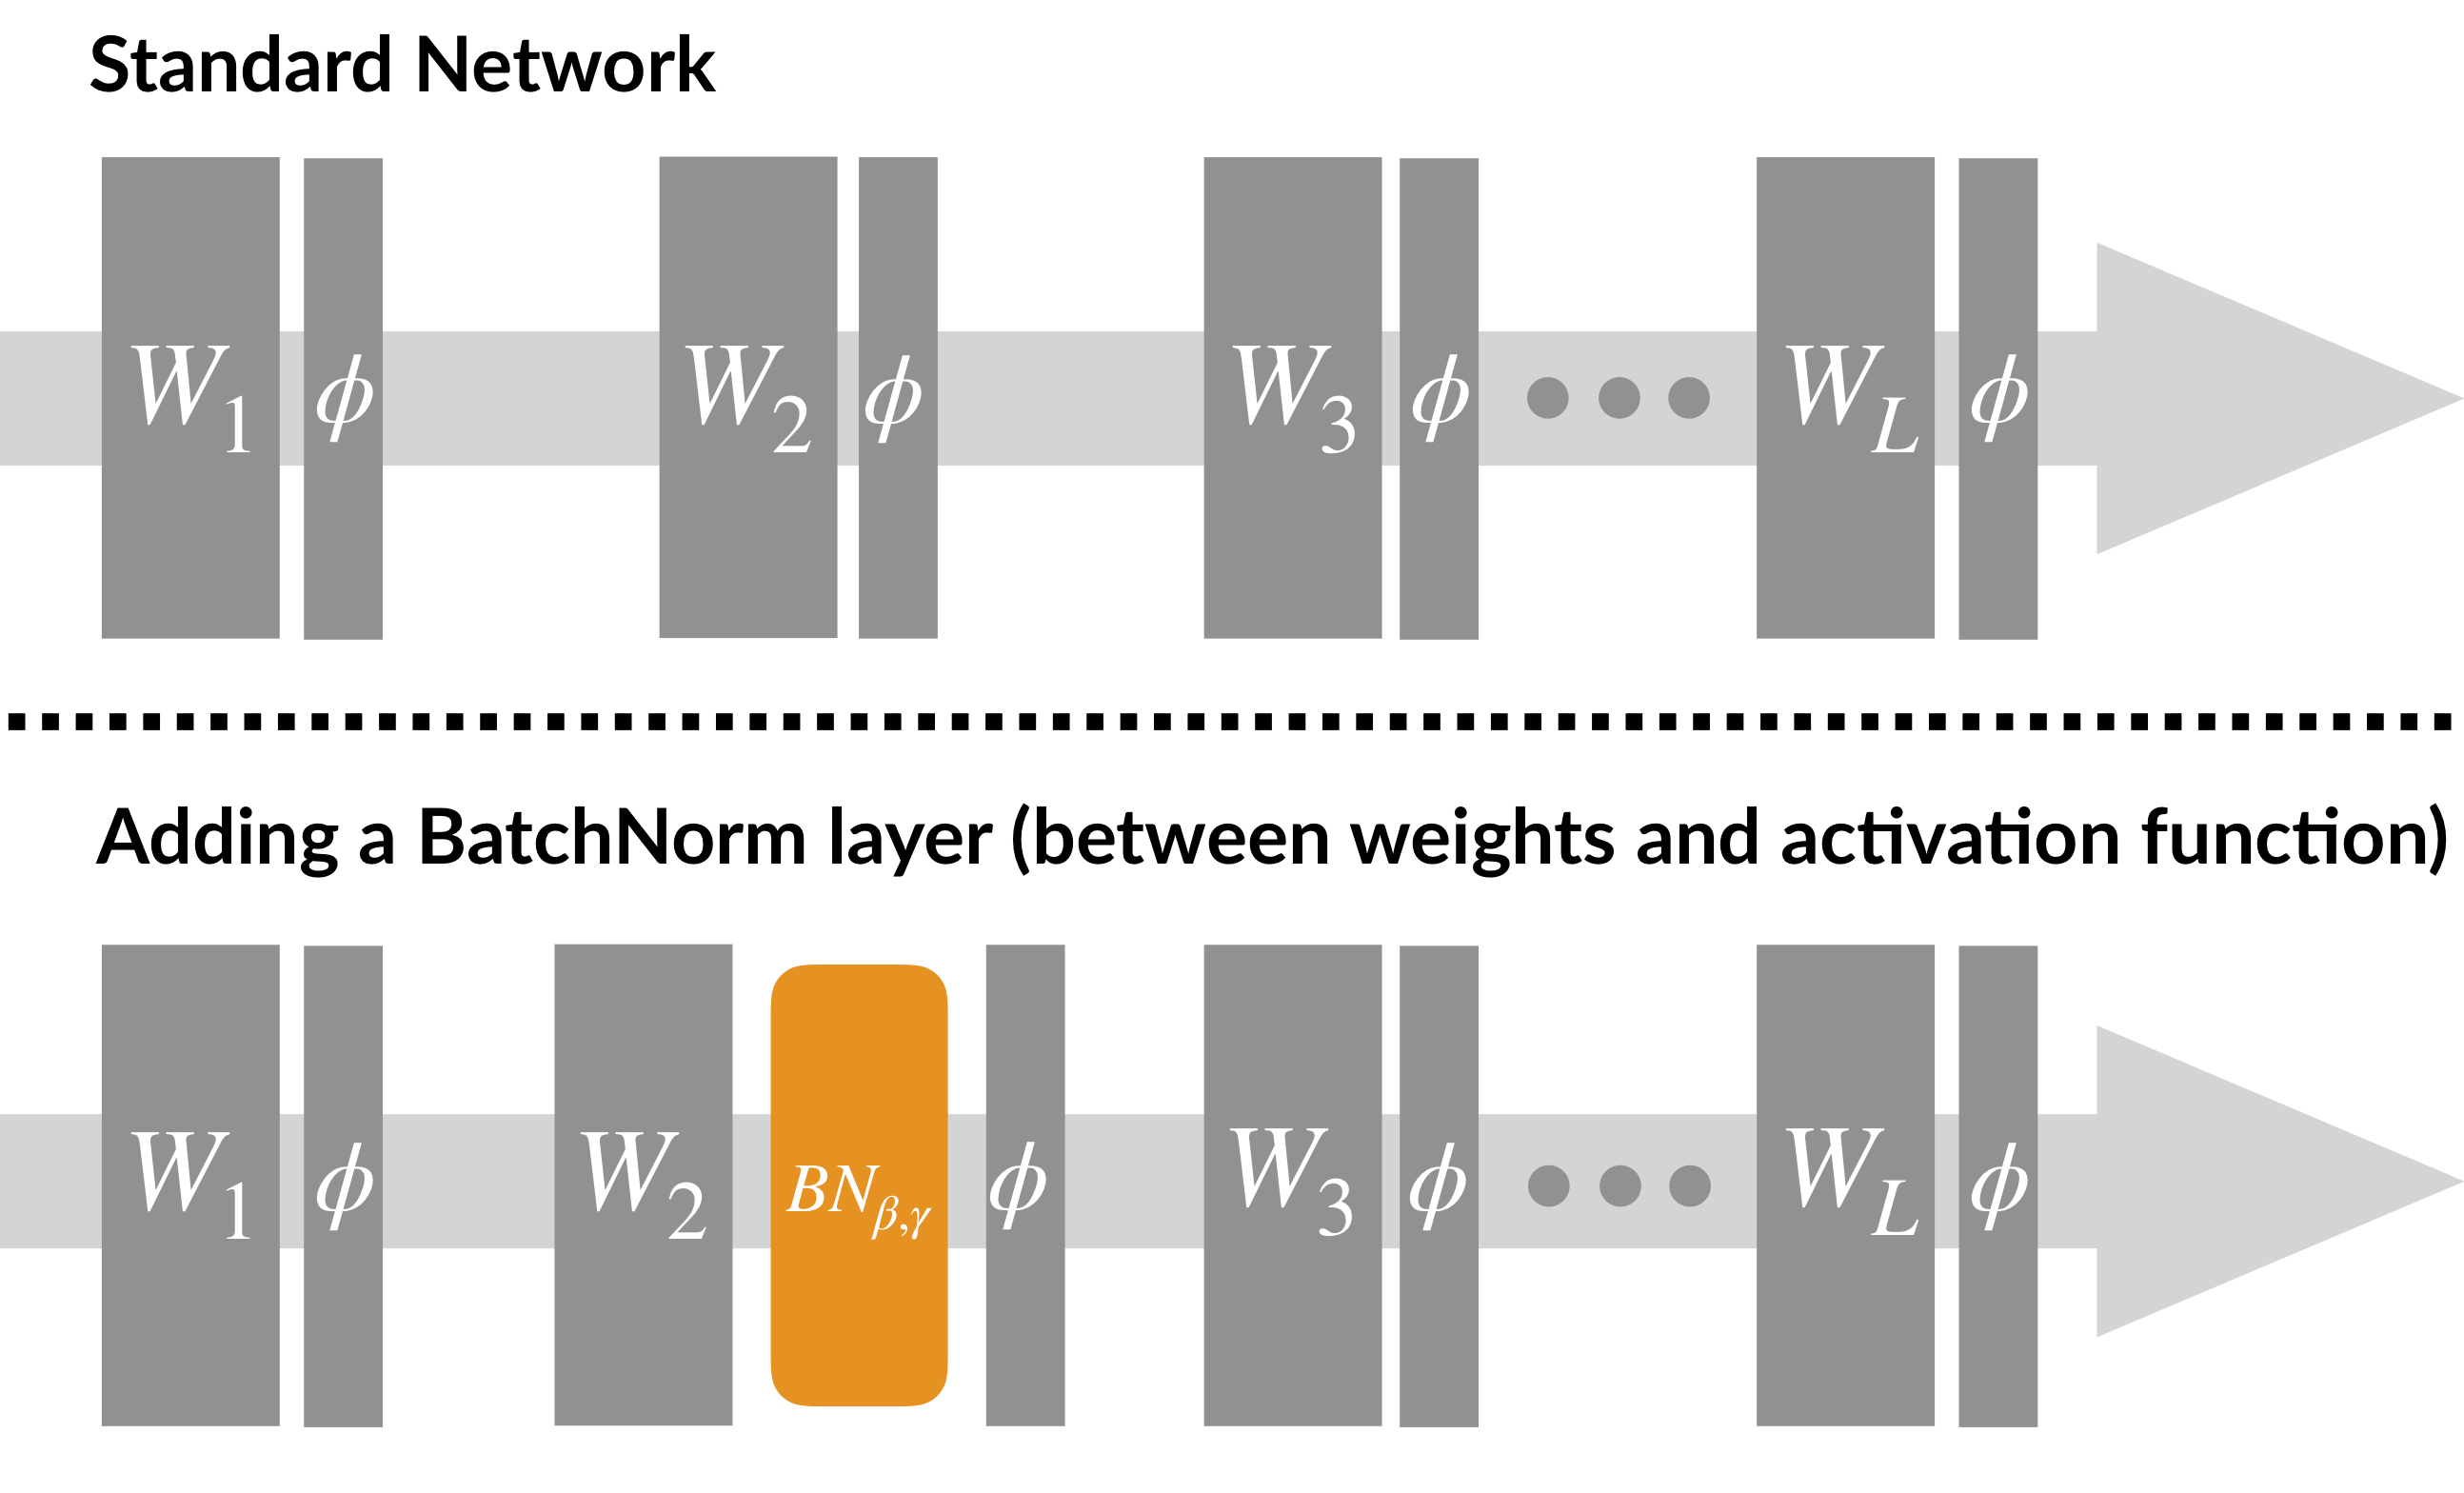
\includegraphics[width=0.75\textwidth]{Figs/section_4/batchnorm_2.jpg}
		\caption{The suggested place to put a BatchNorm layer, \href{https://gradientscience.org/batchnorm/}{Source}}
	\end{figure}
\end{frame}
\begin{frame}{Batch Norm: Training Time}
	\begin{itemize}
		\item First, it zero-centers and normalizes the batch.
	\end{itemize}
	\vspace{0.05\textheight}
	\begin{equation*}
		\mathlarger{
			\mu_B := \frac{1}{N_B} \sum{x_B^{(i)}}
		}
	\end{equation*}
	\begin{equation*}
		\mathlarger{
			\sigma_B^2 := \frac{1}{N_B} \sum{(x_B^{(i)} - \mu_B)^2}
		}
	\end{equation*}
	\begin{equation*}
		\mathlarger{
			\hat{x_B}^{(i)} = \frac{x_B^{(i)} - \mu_B}{\sqrt{\sigma^2_B + \epsilon}}
		}
	\end{equation*}
	\begin{itemize}
		\item Then, scales and shifts the batch with two learnable parameters $\gamma, \beta$.
	\end{itemize}
	\vspace{0.05\textheight}
	\begin{equation*}
		\mathlarger{
			y_B^{(i)} = \gamma \hat{x_B}^{(i)} + \beta	
		}
	\end{equation*}
\end{frame}
\begin{frame}{Batch Norm: Test Time}
	\begin{itemize}
		\item To zero-center and normalize the input, we need the average and variance of the whole data.
		\medskip
		\item Those parameters can be acquired during the training.
		\medskip
		\item Therefore, we need two more trainable parameters.
	\end{itemize}
	\vspace{0.1\textheight}
	\begin{equation*}
		\mathlarger{
			\mu_D := \frac{1}{N} \sum{x^{(i)}}
		}
	\end{equation*}
	\begin{equation*}
		\mathlarger{
			\sigma_D^2 := \frac{1}{N} \sum{(x^{(i)} - \mu_D)^2}
		}
	\end{equation*}
\end{frame}
\begin{frame}{Batch Norm: Test Time}
	\begin{itemize}
		\item The majority of Batch Normalization implementations use an exponential moving average of the layer's input means and standard deviations to estimate these final statistics during training.
	\end{itemize}
	\begin{align*}
		\scalebox{1.5}{$\mu_D $} & \scalebox{1.5}{$= \alpha \mu_D + (1 - \alpha) \mu_B$} \\
		& \scalebox{1.5}{$= \mu_D - (1 - \alpha) \mu_D + (1 - \alpha) \mu_B$} \\
		& \scalebox{1.5}{$= \mu_D - (1 - \alpha)(\mu_D - \mu_B)$}
	\end{align*}
	\begin{itemize}
		\item $\alpha$ is the momentum hyperparameter.
		\medskip
		\item Based on the equations, older values are lost earlier when momentum is less. 
		\item As a result, the moving average changes more quickly.
	\end{itemize}
\end{frame}
\begin{frame}{Batch Norm: Performance}
	\begin{itemize}
		\item Normalizing the data improves the convergence speed by a considerable amount.
	\end{itemize}
	\begin{figure}[H]
		\centering
		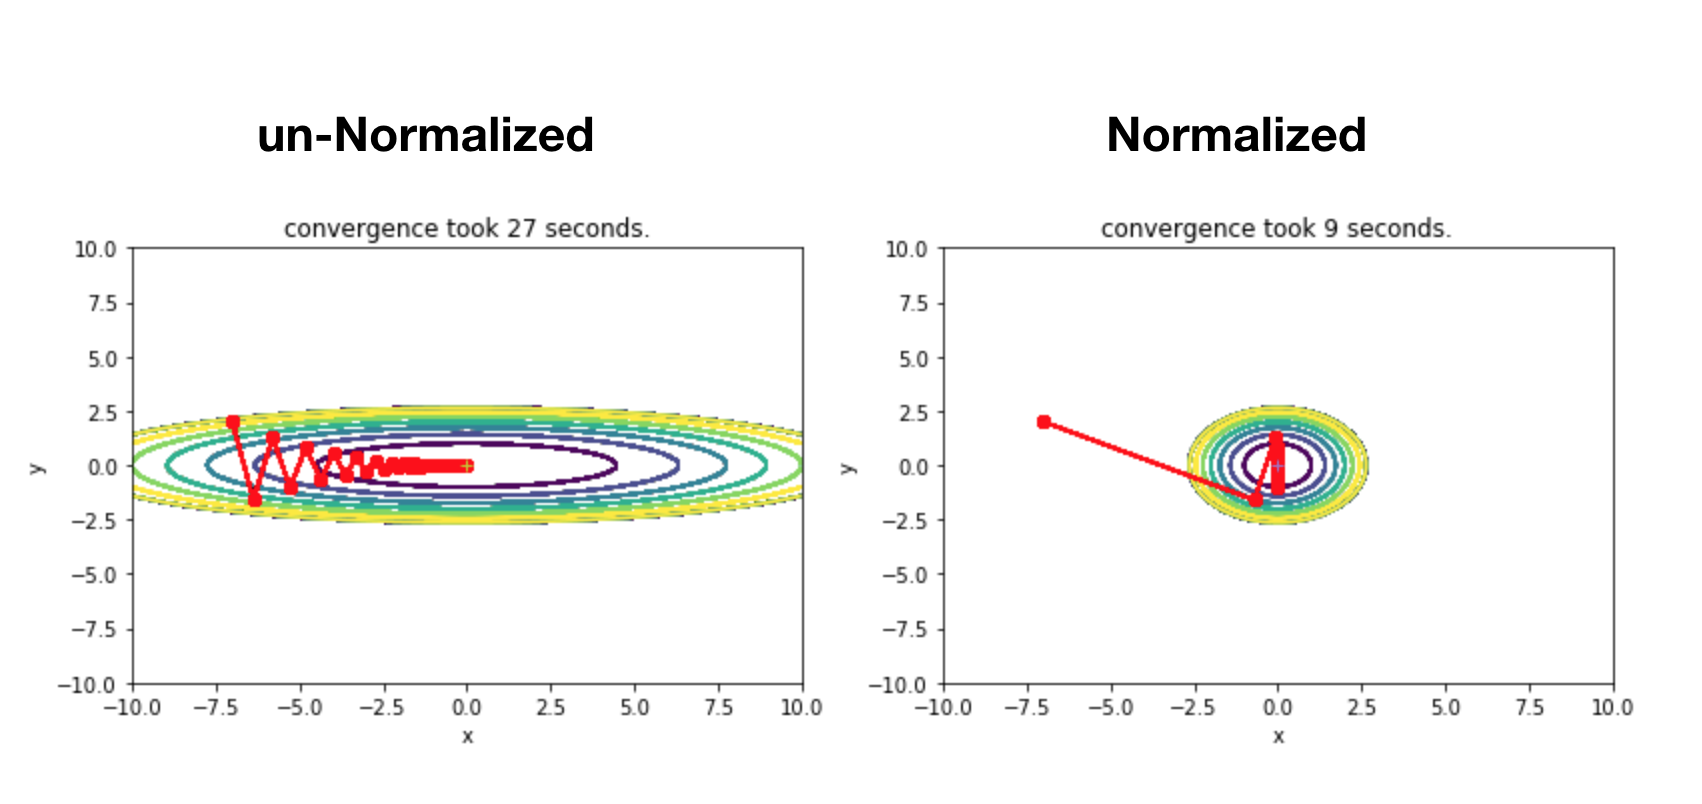
\includegraphics[width=0.8\textwidth]{Figs/section_4/batchnorm_3.png}
		\caption{BatchNorm performance. Convergence speed is increased by 200\%,  \href{https://jsideas.net/batch_normalization/}{Source}}
	\end{figure}
\end{frame}
\begin{frame}{Batch Norm}
	\begin{itemize}
		\item Pros
		\medskip
		\begin{itemize}
			\item Vanishing/Exploding gradient problem is reduced by a considerable amount.
			\medskip
			\item You can use even saturating activation functions.
			\medskip
			\item The network is much less sensitive to the initial weight.
			\medskip
			\item We're able to use larger learning rates, which speeds up the training.
			\medskip
			\item It also acts as a regularizer.
			\medskip
			\begin{itemize}
				\item There is no need for other regularizer techniques.
			\end{itemize}
		\end{itemize}
	\end{itemize}
\end{frame}
\begin{frame}{Batch Norm}
	\begin{itemize}
		\item Cons
		\begin{itemize}
			\item It increases model parameters and prediction latency.
			\medskip
		\end{itemize}
	\end{itemize}
	\begin{itemize}
		\item Solution: during the test time, we can mix the BatchNorm layer with its previous layer to hold the prediction latency.
	\end{itemize}
	\begin{columns}
		\begin{column}[c]{0.45\textwidth}
			\centering
			\begin{equation*}
				\mathlarger{x'^{(i)} = W x^{(i)} + b}
			\end{equation*}
			\begin{equation*}
				\mathlarger{y^{(i)} = \frac{x'^{(i)} - \mu_D}{\sqrt{\sigma_D^2 + \epsilon}} + \beta}
			\end{equation*}
		\end{column}
		\begin{column}[c]{0.1\textwidth}
			\centering
			\begin{equation*}
				\mathlarger{\mathlarger{
						\Rightarrow
				}}
			\end{equation*}
		\end{column}
		\begin{column}[c]{0.45\textwidth}
			\centering
			\begin{equation*}
				\mathlarger{y^{(i)} = W' x^{(i)} + b'}
			\end{equation*}
			\begin{equation*}
				\mathlarger{
					W' := \frac{1}{\sqrt{\sigma_D^2 + \epsilon}} W	
				}
			\end{equation*}
			\begin{equation*}
				\mathlarger{
					b' := \beta + \frac{b- \mu_D}{\sqrt{\sigma_D^2 + \epsilon}}	
				}
			\end{equation*}
		\end{column}
	\end{columns}
\end{frame}